\chapter{Literature Review}\label{Literature Review}

In this chapter we will build on the background in the previous chapter to give a critical review of previous work applying subspace learning algorithms and the existing problems.


\section{Applications of Subspace Learning Algorithms in Biomedical Data}
section{Applications to Neuroimaging}

There have been a number of applications of CCA and related methods to multiview problems in neuroimaging. Using resting state fMRI data, modes of correlation have been found that relate to differences in sex and age relating to drug and alcohol abuse, depression and self harm \cite{mihalik2019brain}. A similar mode relating to `positive-negative' wellbeing has been found across studies \cite{smith2015positive} suggesting that mental wellbeing has a relationship (though not necessarily causally) with functional connectivity between networks in the brain. Later in this dissertation we will replicate and build on the findings from this paper by using regularised and non-linear CCA methods.

CCA has also been used as a preprocessing step in order to identify groups of subjects in the latent variable space. In particular, CCA and clustering have been used to identify depression using fMRI data \cite{dinga2019evaluating} \cite{drysdale2017resting}. CCA has also been used in the manner we described to denoise two views of a dataset such as separate measures of neuroimaging data \cite{zhuang2020technical} to remove artefacts. Deep CCA has recently been used to extract features for the diagnosis of schizophrenia \cite{qi2016deep}.


\section{Regularized CCA, PLS, and PCA}
In this section we review some existing regularised CCA methods including some of the existing extensions to data with more than two views. Since almost all of the existing work considers sparsity inducing regularisation this is the main focus.

There have been many different proposals in the literature for finding sparse regularised solutions. In this section, we describe the penalized matrix decomposition method (arguably the most common in applied sparse CCA) as well as some of the methods based on least squares formulations. Like the unregularised CCA and PLS formulations, they can broadly be grouped into penalized SVD based methods and penalised iterative methods.

\subsection{Penalized Matrix Decomposition}\label{sec:witten}

Witten's "Penalized Matrix Decomposition" (PMD) \cite{witten2009penalized} approach substitutes the CCA constraints $\bold{w_i^{\top}X_i^{\top}X_iw_i}=1$ for the PLS constraints $\bold{w_i^{\top}w_i}=1$. This is equivalent to assuming that the variance-covariance matrix of $X$ is an identity matrix or in other words that the columns of the original data matrices are independent. This subtle change means that Witten's method introduced in this paper is only an approximation to a sparse CCA optimisation problem. It follows that this method will perform best (in terms of optimising the `true' CCA objective) when the identity covariance matrix assumption is strongest. In addition, much as with PLS, PMD is biased towards the largest principal components in the data and will select directions with high covariance even if they are not the maximally correlated directions.

Since the PLS constraint $\bold{w_1^{\top}w_1}=1$ is non-convex, Witten further relaxes this constraint to an inequality. The penalized matrix decomposition can then be expressed as the constrained optimization problem in \ref{eq:pmd}.

\begin{align}
    \label{eq:pmd}
    & \bold{w_{opt}}=\underset{\bold{w}}{\mathrm{argmax}}\{ \bold{w_1^{\top}X_1^{\top}X_2w_2} \}\\
    & \text{subject to:} \notag\\
    & \bold{w_1^{\top}w_1}\leq1 \notag\\
    & \bold{w_2^{\top}w_2}\leq1 \notag\\
    & P(\bold{w_1})\leq c_1 \notag\\
    &P(\bold{w_2})\leq c_2 \notag
\end{align}

Where $P(\bold{w_1})=\|\bold{w_1}\|_1$ would form a constraint on the 1-norm but in principle the algorithm only requires that $P(\bold{w_1})$ is a one-homogenous function:

\begin{align}
    & \lambda P(\bold{w})=P(\lambda \bold{w})
\end{align}

In order to solve this optimisation, Witten proposed an algorithm based on a rank 1 singular value decomposition of a matrix $\bold{M}=\bold{X_1^{\top}X_2}$. Since soft-thresholding is equivalent to Lasso when $\bold{X_i^{\top}X_i}=\bold{I}$, the algorithm is simply the power method for singular value decomposition with soft-thresholding applied at each iteration such that $\|\bold{w_i}\| \leq c_i$. The soft-threshold function can be written as:

\begin{align}
    \label{eq:softthreshold}
    & S(x,\gamma) = \text{sign}(x)\text{max}(0,\|\bold{x}\|-\gamma)
\end{align}

Where $\gamma$ defines the threshold of the absolute value below which coefficients in $x$ are set to zero. We can then iteratively find the threshold $\gamma$ that fulfils the l1-norm condition using for example binary search:

\vspace{\baselineskip}
\begin{algorithm}[H]
    \begin{algorithmic}
        \STATE {Finds local optima for sparse left and right eigenvectors of the covariance matrix} $X_1^{\top}X_2$
        \STATE $M_1=X_1^{\top}X_2$
        \FOR {$k \gets 1$ \textbf{to} $K$}
        \STATE Initialize $|w^{(k)}_2|_2=1$
        \WHILE {Not converged}
        \STATE $w^{(k+1)}_1=M_kw^{(k)}_2$
        \STATE $w^{(k+1)}_1=S(w^{(k+1)}_1,\gamma)$
        \STATE $w^{(k+1)}_1=\frac{w^{(k+1)}_1}{\|w^{(k+1)}_1\|_2}$
        \STATE $w^{(k+1)}_2=M_k^{\top}w^{(k+1)}_1$
        \STATE $w^{(k+1)}_2=S(w^{(k+1)}_1,\gamma)$
        \STATE $w^{(k+1)}_2=\frac{w^{(k+1)}_2}{\|w^{(k+1)}_2\|_2}$
        \STATE $M_{k+1}=M_k-du_kv_k^{\top}$
        \ENDWHILE
        \ENDFOR
        \caption[Penalized Matrix Decomposition]{Penalized Matrix Decomposition for CCA}
    \end{algorithmic}
\end{algorithm}
\vspace{\baselineskip}

Witten also showed that the lasso constraint could be replaced with a fused lasso constraint by replacing the soft-threshold with an appropriate update step.

\subsection{Penalized CCA}

Parkhomenko proposed a similar algorithm to penalized matrix decomposition, substituting the covariance matrix $\bold{X_1^{\top}X_2}$ for the correlation matrix $\bold{(X_1X_1^{\top})^{-\frac{1}{2}}X_1^{\top}X_2(X_2^{\top}X_2)^{-\frac{1}{2}}}$\cite{parkhomenko2009sparse}. However their soft-thresholding step uses the threshold as the hyper-parameter and therefore cannot be written as a constrained optimization problem. For this reason it is also difficult to select an appropriate range for the hyperparameters $\gamma_i$ as this is more dataset dependent:

\begin{align}
    \label{eq:parkho}
    & \bold{w_{opt}}=\underset{\bold{w}}{\mathrm{argmax}}\{ \bold{(X_1X_1^{\top})^{-\frac{1}{2}}X_1^{\top}X_2(X_2^{\top}X_2)^{-\frac{1}{2}}} \}
\end{align}

While this makes the optimisation more CCA-like than PLS-like, it requires us to calculate the inverses $\bold{(X_1X_1^{\top})^{-\frac{1}{2}}}$ and $\bold{(X_2^{\top}X_2)^{-\frac{1}{2}}}$. However in cases where the number of features $p$ is greater than the number of samples $n$, as is common in many applications of sparse modelling such as neuroimaging, these matrices cannot be inverted.

For this reason, Parkhomenko recommended diagonalising the covariance matrices $\bold{X_i^{\top}X_i}$ or making them identity matrices. Witten's method can thus be seen as an extremely regularised version of Parkhomenko's.

\subsubsection{Alternating Least Squares}\label{sec:ALS}

Since the scale invariance constraints in the CCA optimisation problem can also be represented by the unconstrained objective:

\begin{align}
    & \bold{w_{opt}}=\underset{\bold{w}}{\mathrm{argmax}}\{\bold{\frac{\bold{w_1^{T}X_1^{T}X_2w_2}}{\|\bold{X_1w_1}\|_{2}\|\bold{X_2w_2}\|_{2}}}\}
\end{align}

And since by adding constants to the objective we can show that maximising the objective is equivalent to minimising the distance between the two normalized projections \cite{golub1995canonical}:

\begin{align}
    \left\|\bold{\frac{X_1 w_1}{\|X_1 w_1\|_{2}}-\frac{X_2 w_2}{\|X_2 w_2\|_{2}}}\right\|_{2}^{2}=2\left(1-\bold{\frac{w_2^{T} X_2^{T} X_1 w_1}{\|X_2 w_2\|_{2}\|X_1 w_1\|_{2}}}\right)
\end{align}

We can transform the problem of maximising correlation to one of minimising the distance between the normalized projections $\bold{X_1w_1}$ and $\bold{X_2w_2}$.

This optimisation problem is convex in one variable when the other variable is fixed. Problems of this kind are referred to as biconvex (in the two variable case) and multiconvex (where it is true for more than two variables). They are typically optimized by iterating between these two convex problems, successively fixing $\bold{w_1}$ and solving for $\bold{w_2}$ and vice versa. This is referred to in this case as the "alternating least squares" method \cite{lykou2010sparse}.

It is known that the alternating least squares algorithm is slower to converge when the 1st and 2nd canonical correlations (singular values of the covariance matrix $\bold{X_1^{\top}X_2}$) are closer together \cite{venkatg}.

\subsection{Iterative Penalized Least Squares for Sparse CCA}

There have been some proposals for sparse CCA that relate to the alternating regression form of CCA. Wilms originally proposed "sparse alternating regressions" \cite{wilms2015sparse} which replace the least squares problems at each iteration with lasso penalized regressions and a normalization step as shown in equation \ref{eq:SAR}:

\begin{align}
    \label{eq:SAR}
    & \bold{\hat{w}^{(i+1)}_1}=\underset{\bold{w}}{\mathrm{argmin}}\{ \|\bold{Xw-y}\|^2_2 + \lambda\|\bold{w}\| \}\\
    & \bold{w^{(i+1)}_1}=\bold{\frac{\hat{w}^{(i+1)}_1}{\|\hat{w}^{(i+1)}_1\|}}
\end{align}

It is clear that when the regularisation parameters $\lambda$ are set to zero we recover the alternating least squares CCA formulation.

Mai offered a proof that the sparse alternating regression normalization step gave a true global solution to a projection-length constrained lasso regression\cite{mai2019iterative}:

\begin{align}
    & \bold{w}=\underset{\bold{w}}{\mathrm{argmin}}\{ \|\bold{Xw-y}\|^2_2 + P(\bold{w}) \}\\
    & \text{subject to:} \notag\\
    & \bold{w^{\top}X^{\top}Xw}=1 \notag
\end{align}

Furthermore, Mai showed that in principle the lasso penalty could be replaced with any one homogenous regularisation functional. The proof is sketched out as below:

\begin{thm}

    For one-homogenous function $P(x)$, if the solution $\bold{\hat{w}}$ satisfies the unconstrained problem:

    \begin{align}
        & \bold{\hat{w}}=\underset{\bold{w}}{\mathrm{argmin}}\{ \|\bold{Xw-y}\|^2_2 + P(\bold{w}) \}
    \end{align}

    Then the solution $\bold{w}$ to the constrained problem:

    \begin{align}
        & \bold{w}=\underset{\bold{w}}{\mathrm{argmin}}\{ \|\bold{Xw-y}\|^2_2 + P(\bold{w}) \}\\
        & \text{subject to:} \notag\\
        & \bold{w^{\top}X^{\top}Xw}=1 \notag
    \end{align}

    is equal to $\bold{w}=\bold{\frac{\hat{w}}{\|X\hat{w}\|}}$ or $\bold{w}=\bold{(\hat{w}^{\top}X^{\top}X\hat{w})^{-\frac{1}{2}}\hat{w}}$

\end{thm}

\begin{proof}

    We have $c^2=\bold{\hat{w}^{\top}X^{\top}X\hat{w}}$. By definition we must also have $1=(c^{-1}\bold{\hat{w}^{\top})X^{\top}X(c^{-1}\hat{w})}$. Mai notes that the solution $\bold{\hat{w}}$ must also satisfy a constrained optimisation problem:

    \begin{align}
        & \bold{\hat{w}}= \underset{\bold{w}}{\mathrm{argmin}}\{ \|\bold{Xw-y}\|^2_2 + P(\bold{w}) \}\\
        & \text{subject to:} \notag\\
        & \bold{w^{\top}X^{\top}Xw}=c \notag
    \end{align}

    By substituting the constraints, Mai shows that this is the same as finding:

    \begin{align}
        & \bold{\hat{w}}=\underset{\bold{w}}{\mathrm{argmin}}\{ -\bold{y^{\top}Xw} + P(\bold{w)} \}\\
        & \text{subject to:} \notag\\
        & \bold{w^{\top}X^{\top}Xw}=c \notag
    \end{align}

    Where $c=1$ for the unit length constrained problem. Mai then defines:

    \begin{align}
        & J(\beta)=-\bold{y^{\top}Xw} + P(\bold{w})\\
    \end{align}

    and uses the chain of inequalities:

    \begin{align}
        \label{eq:maiinequalitychain}
        & J(\bold{w}) \leq J(c^{-1}\bold{\hat{w}})=c^{-1}J(\bold{\hat{w}}) \leq c^{-1}J(c^{-1}\bold{w}) = J(\bold{w})
    \end{align}

    To show that $J(c^{-1}\hat{\beta})=J(\beta)$.

\end{proof}

\subsection{Elastic Penalized CCA}

In neuroimaging applications, we typically encounter highly correlated variables in the raw data. Since the sparse methods discussed so far may only select one of a number of highly correlated variables, a well known property of the lasso penalty, we may lose out on parts of the interpretability of the model. Waiijenborg proposed the use of elastic net regularisation in order to ensure group-level sparsity using the updates \cite{waaijenborg2008quantifying}:

\begin{align}
    & \bold{\hat{w}^{(i+1)}_1}=\underset{\bold{w_1}}{\mathrm{argmin}}\{(1+\lambda^{(1)}_2)\|\bold{X_1w_1-X_2w^{(i)}_2}\|^2_2 + \lambda^{(1)}_2\|\bold{w_1}\|^2_2 + \lambda^{(1)}_1\|\bold{w_1}\|_1 \}\\
    & \bold{\hat{w}^{(i+1)}_2}=\underset{\bold{w_2}}{\mathrm{argmin}}\{(1+\lambda^{(2)}_2)\|\bold{X_1w_1^{(i)}-X_2w_2}\|^2_2 + \lambda^{(2)}_2\|\bold{w_2}\|^2_2 + \lambda^{(2)}_1\|\bold{w_2}\|_1 \}
\end{align}

Where $\bold{\hat{w}}$ denotes unnormalized weights which are normalized in the same way as \ref{eq:SAR}. While the algorithm produces good results in practice, it has no theoretical guarantee of convergence or optimality and cannot simply be written as an optimization problem. In particular, as we showed in the previous section, normalizing the solutions to the unconstrained update equations in order to fulfil the projection-length constraint does not guarantee that we find a global optimum for the constrained optimization.


\section{Large scale CCA, PLS, and PCA}

\textbf{Stochastic GEPs}
Several methods have been proposed for solving GEPs with SGD.
\cite{arora2017stochastic} developed a Matrix Stochastic Gradient (MSG) method for finding the top-k CCA subspace, however its tractability relies on using minibatches of size 1. \cite{chen2019constrained} proposed a subspace Generalized Hebbian Algorithm (SGHA) which requires Lagrange multipliers. \cite{xie2015scale} propose a similar class of algorithms, but which estimate directions sequentially rather than as a subspace; \cite{chapman2022generalized} show there are also pseudo-objective based methods corresponding to this class of algorithms. More recently, the EigenGame line of work \cite{gemp20,gemp2021} has reframed the top-k subspace problem as a competitive game between components and recently extended the work to GEPs \cite{gemp2022generalized}. To our knowledge these are the state-of-the-art. However, there has been extensive other work tackling the top-1 problem in the stochastic CCA as well as stochastic PCA and PLS \cite{arora2012stochastic,arora2016stochastic,arora2017stochastic}.


\section{Deep CCA, PLS, and PCA}

\subsection{Deep Learning}

With large amounts of data and improvements in hardware in recent years, `Deep' neural networks have become the state of the art in many tasks and in particular in computer vision. In principle, an infinitely wide neural network could model any function to arbitrary accuracy - a property known as the universal approximation theorem - and this flexibility allows neural networks to model complex relationships.

In practice, rather than infinitely wide networks, `Deep' Neural Networks combine layers of linear weights with non-linear activation functions. Each layer can generally be written as a function of the outputs of the previous layer (or the raw input for the first layer):

$$
\bold{h_i}=s_i(\bold{W_ih_{i-1}}+\bold{b_i})
$$

Where we use the letter $h$ to denote a `hidden' layer or a representation between the input and output, $W$ to represent a matrix of weights, $b_i$ to represent a vector of bias terms and $s$, critically, to represent a non-linear activation function. One example of a non-linear activation function is the sigmoid function which maps linear outputs to a value between 0 and 1. Neural networks are often designed to have bottlenecks with fewer features in each subsequent hidden layer. This means that the outputs of each layer produce a hierarchy of features and it is often hypothesized that their generalisation ability is built upon producing these layers of abstraction\cite{li2018survey}. In general we will refer to the complete set of parameters (and architectural choices such as the number of layers) in a neural network with $\theta$. We therefore write a neural network function as $F(\bold{X};\theta_F)$.

The most common way to optimize neural networks is to use gradient descent (GD) in which we calculate the gradient of the network parameters with respect to some objective. When using the whole dataset to calculate the gradient we typically refer to `batch' gradient descent. However, when using non-linear functions, the objective is typically non-convex meaning GD is prone to finding local minima (regions in the parameter space where the gradient of the objective is zero) rather than global minima (local minima where the value of the objective is optimal). Perhaps for this reason, it is more effective to use Stochastic Gradient Descent (SGD), in which we estimate the gradient by using a single sample or a small set of samples referred to as a `minibatch'. This noisy estimate is less likely to get `stuck' in suboptimal solutions. Stochastic gradient descent mathematically relies on the stochastic estimate of the gradient being an unbiased estimate of the true gradient.

\subsection{Deep CCA}

Deep Canonical Correlation Analysis provides an alternative method to kernel CCA for finding complex non-linear structure in multiview data \cite{andrew2013deep}. In Deep CCA we look to use functions parameterized by neural networks $F(\bold{X};\theta_F)$ and $G(\bold{Y};\theta_G)$ to map the original data into a space in which the two views are maximally correlated. The problem we would like to solve is therefore:

\begin{align}
    & \theta_{F_{opt}},\theta_{G_{opt}}=\mathrm{argmax}\{\text{trace}( F(\bold{X};\theta_F)^{\top}G(\bold{Y};\theta_G))  \}\\
    & \text{subject to:} \notag\\
    & F(\bold{X};\theta_F)^{\top}F(\bold{X};\theta_F)=1 \notag\\
    & G(\bold{Y};\theta_G)^{\top}G(\bold{Y};\theta_G)=1 \notag
\end{align}

As we showed earlier in section \ref{sec:cca}, sum of the top $k$ canonical correlations of two views of a dataset can be shown to be the sum of the top $k$ singular values of the matrix $\bold{T}=\bold{\Sigma_{11}^{-\frac{1}{2}}\Sigma_{12}\Sigma_{22}^{-\frac{1}{2}}}$ where $\Sigma_{11}=F(\bold{X};\theta_F)^{\top}F(\bold{X};\theta_F)$. Now consider the identity $\|\bold{T}\|_*=\text{tr}(\sqrt{\bold{T^{\top}T}})$ known as the tracenorm of $\bold{T}$. This is symmetric and therefore can be diagonalised. Then since $T=\bold{U\Sigma V^{\top}}$:

\begin{align}
    & \|\bold{T}\|_*=tr(\sqrt{\bold{V\Sigma U^{\top}U\Sigma V^{\top}}})=tr(\sqrt{\bold{\Sigma^2 VV^{\top}}})=tr(\bold{\Sigma})
\end{align}

Therefore maximising the tracenorm maximises the total correlation between the representations.

\begin{figure}[H] %[H] "corresponds to start the figure Here"
    \centering %alignment can be flushleft, centering or flushright
    %includegraphics is the command to include graphics or pictures, [Width should be defined with respect to textwidth]{The path/ location of the image in the specified folder}, the image should be either in .png, .jpg, .pdf formats faster processing
    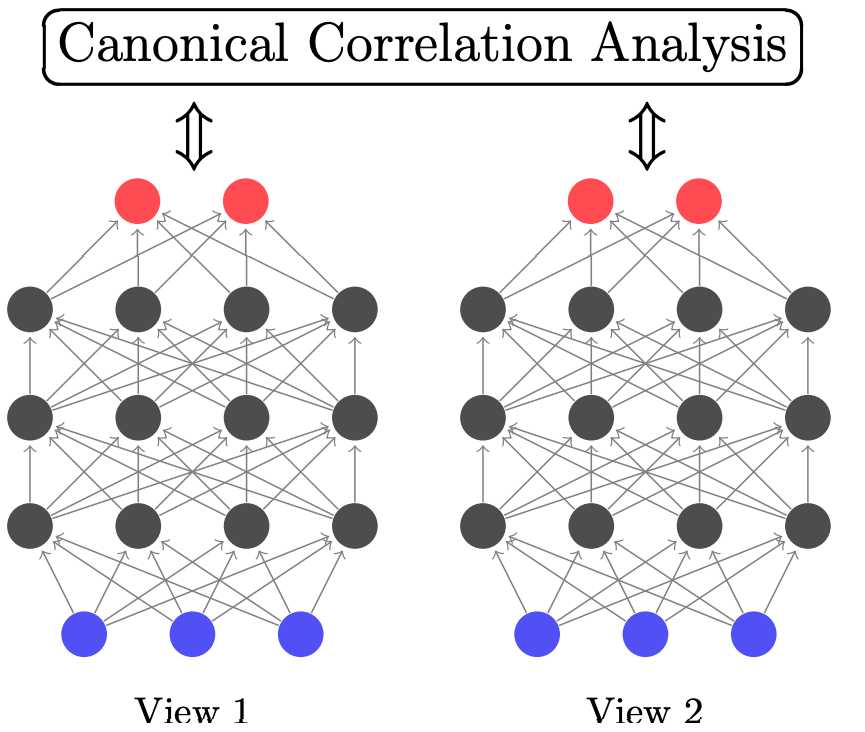
\includegraphics[width=0.5\textwidth]{chapters/litreview/DCCA.png}
    \caption[Deep CCA Representation]{\textit{\textbf{Deep CCA with two correlated dimensions:}} A separate neural network is learnt for each view and a linear CCA is applied on top \cite{andrew2013deep}}
    \label{img:DCCA}
\end{figure}

A major problem with this DCCA formulation is that it relies on full-batch optimisation (optimized in the original paper by using the L-BFGS optimization algorithm). When gradients are calculated using smaller minibatches, the performance degrades drastically because the estimation of the gradient is biased. In particular, mathematically the terms in $\Sigma_{ii}^{-\frac{1}{2}}$ are overestimated due to Jensen's inequality $E[\frac{1}{X}]>\frac{1}{E[X]}$. More intuitively, these matrices may be near singular for small samples causing stochastic gradients to blow up.


\section{Self-Supervised Learning}

\subsubsection{Barlow Twins}
%Relationship to CCA

\subsubsection{VICReg}
%Likewise


It is well known that VICReg and Barlow twins are closely related to CCA \cite{balestriero2022contrastive}. Similarly, \cite{kiani2022joint} showed how the SSL losses like VICReg could be adapted and implemented in closed form using the kernel method. Our work approaches the problem from the opposite angle, demonstrating how these classical problems can be extended to deep learning and solved with SGD without introducing bias.


\section{Summary}